% CFP: https://discourse.llvm.org/t/cfp-llvm-hpc-workshop-at-sc-25/86391
% At least 5 two-column pages, excluding the bibliography and figures

% Submission: Aug 15, 2025
% Internal deadline: Aug 4, 2025

% CFP:
% Paper submissions due: August 15, 2025 (AoE)
% Notification to authors of acceptance: September 5, 2025
% Camera-ready papers due: September 29, 2025
% Workshop takes place: November 17, 2024

% Topics:
% 1) The LLVM IR generated by OpenMPIRBuilder can be easily optimized by OpenMPOpt pass (the old flang cannot do it)
% 2) The support of math functions for AMDGPU is done by MLIR code which is also used for GPU-specific optimization for other workloads.
% 3) We can reuse AMD downstream NO_LOOP mode which was written for OpenMP C for Fortran (in progress, but the tests show that it's beneficial)

% Detailed plan for #2 proposal:

% General issues:
% Terminology:
%   array descriptor vs dope vector? -> array descriptor
% Default compiler:
%   AOMP Flang/upstream flang? -> AMD Flang, AFAR builds
% Default GPU?
% Are we allowed to present some numbers from microbenchmarks? (i.e. very small code snippets used only for illustration of the problem)

% 1) Handling of descriptors of Fortran pointers and allocatable arrays (The code with allocatable arrays requires more resources in comparison to stack arrays)
%  -> Fortran differences between static and dynamic arrays vs C:
%     a) static -> the size is known in compilation time
%     b) dynamic -> the size and shape is unknown in compilation time
%     c) allocate vs malloc in C
%        * allocate -> defines the shape and size of the allocated array. The information about size/shape and the beginning of allocated memory is stored in array descriptor.
%        * malloc -> allocates N consecutive bytes and it returns address of the first byte
%  -> MLIR(HLFIR + FIR)+LLVM IR code analysis of simple operation a[i] = 5 for static and dynamic arrays for code:
%  !$omp target teams distribute parallel do map(tofrom: x)
%  do i = 1, 255
%    x(i) = a(i) + b(i)
%   end do
%     a) host side + mapping
%     b) GPU side
%  -> Comparison of required resources for exemplary kernels: SGPRS/VGPRS for different optimization levels (are we allowed?)

% 2) Problems related to temporary arrays (i.e.: iaVS = [ iV, jV, kV ] + iaS ) and option -fstack-arrays as remedy.
%  -> Flang default handling of temporary arrays (heap allocation)
%  -> Example of usage of temporary array inside GPU code
%  -> Explanation how heap array is handled inside GPU kernel (slow malloc call)
%  -> Explanation of option -fstack-arrays
%  -> Advantages and disadvantages of option -fstack-arrays (Possible stack overflow vs faster GPU kernels)
%  -> Comparison of execution times for kernel with temporary array with and without -fstack-array (are we allowed?)

%% Lower priority, only as space and time permits:
%% 3) The Fortran runtime calls which can involuntarily appear in the GPU code
%% -> Description of Fortran runtime
%%  -> Examples of Fortran code where Fortran runtime is used
%%  -> Consequences of Fortran runtime call inside GPU kernel (are we allowed to present some execution times?)

\documentclass[acmtog,natbib=false]{acmart}
\AtBeginDocument{\providecommand\BibTeX{{Bib\TeX}}}

\RequirePackage[
datamodel=acmdatamodel,
style=acmnumeric, % use style=acmauthoryear for publications that require it
]{biblatex}
\addbibresource{references.bib}

\usepackage[T1]{fontenc}
\usepackage{listings}
\usepackage{minted}
\usepackage{xspace}
\usepackage[printonlyused]{acronym}
\usepackage{xpatch}

%% Rights management information.  This information is sent to you
%% when you complete the rights form.  These commands have SAMPLE
%% values in them; it is your responsibility as an author to replace
%% the commands and values with those provided to you when you
%% complete the rights form.
\setcopyright{acmlicensed}
\copyrightyear{2025}
\acmYear{2025}
\acmDOI{XXXXXXX.XXXXXXX}

%%
%% Submission ID.
%% Use this when submitting an article to a sponsored event. You'll
%% receive a unique submission ID from the organizers
%% of the event, and this ID should be used as the parameter to this command.
\acmSubmissionID{tbd}

%% the listings
\lstset{
  captionpos=b,
}
\setminted{
  escapeinside=||,
  fontsize=\small,
  baselinestretch=0.8,
  linenos,
  numbersep=0.5em,
  xleftmargin=1em
}

%% HACK: fix error marks in minted listings
\makeatletter
\AtBeginEnvironment{minted}{\dontdofcolorbox}
\def\dontdofcolorbox{\renewcommand\fcolorbox[4][]{##4}}
\xpatchcmd{\inputminted}{\minted@fvset}{\minted@fvset\dontdofcolorbox}{}{}
\makeatother

%% useful macros
\newcommand{\todo}[1]{\textcolor{red}{#1}}
\newcommand{\code}[1]{\texttt{#1}\xspace}
\newcommand{\registered}[0]{\textsuperscript{\textregistered}\xspace}
\newcommand{\trademark}[0]{\texttrademark\xspace}

\begin{document}
\title{Implementing OpenMP\registered Offload Support in the AMD Next Generation Fortran Compiler}

\author{Dominik Adamski}
\email{dominik.adamski@amd.com}
\orcid{0009-0008-2698-7516}
\affiliation{%
  \institution{Advanced Micro Devices}
  \city{Łódź}
  \state{Łódzkie Voivodeship}
  \country{Poland}
}

\author{Sergio Afonso}
\email{sergio.afonsofumero@amd.com}
\orcid{0000-0003-0838-8057}
\affiliation{%
  \institution{Advanced Micro Devices}
  \city{Santa Cruz de Tenerife}
  \state{Canary Islands}
  \country{Spain}
}

\author{Akash Banerjee}
\email{akash.banerjee@amd.com}
\orcid{}
\affiliation{%
  \institution{Advanced Micro Devices}
  \city{Milton Keynes}
  \state{England}
  \country{UK}
}

\author{Pranav Bhandarkar}
\email{pranav.bhandarkar@amd.com}
\orcid{0009-0003-3192-330X}
\affiliation{%
  \institution{Advanced Micro Devices}
  \city{Austin}
  \state{TX}
  \country{USA}
}

\author{Kareem Ergawy}
\email{kareem.ergawy@amd.com}
\orcid{0009-0002-6326-8664}
\affiliation{%
  \institution{Advanced Micro Devices GmbH}
  \city{Munich}
  \state{BY}
  \country{Germany}
}

\author{Andrew Gozillon}
\email{andrew.gozillon@amd.com}
\orcid{0000-0001-7558-7166}
\affiliation{%
  \institution{Advanced Micro Devices AB}
  \city{Malmo}
  \state{Skåne County}
  \country{Sweden}
}

\author{Michael Klemm}
\email{michael.klemm@amd.com}
\orcid{0000-0002-8634-4634}
\affiliation{%
  \institution{Advanced Micro Devices GmbH}
  \city{Munich}
  \state{BY}
  \country{Germany}
}

\author{Jan Leyonberg}
\email{jan.leyonberg@amd.com}
\orcid{0009-0001-6657-9719}
\affiliation{%
  \institution{Advanced Micro Devices}
  \city{Toronto}
  \state{ON}
  \country{Canada}
}

\author{Dan Palermo}
\email{dan.palermo@amd.com}
\orcid{0009-0005-7205-2250}
\affiliation{%
  \institution{Advanced Micro Devices}
  \city{Austin}
  \state{TX}
  \country{USA}
}

\renewcommand{\shortauthors}{Adamski et al.}

\begin{abstract}
Modern day supercomputers are massively parallel, heterogeneous systems, many of which employ \acp{GPU} to accelerate applications.
While C/C++, but also Python, gain traction in the \ac{HPC} domain, Fortran continues to have a large developer base with new high performance code written every day.
The OpenMP \ac{API} is a key ingredient to provide multi-threading and support for offloading execution to \acp{GPU}.
AMD is developing the AMD Next Generation Fortran compiler that will eventually replace the existing AMD Fortran Compiler, which is based on the Classic Flang compiler.
This paper describes the general compilation pipeline of the AMD Next Generation Fortran Compiler.
It shows how the compiler generates code for OpenMP \code{target} directives and their \code{map} clauses.
The paper closes with a discussion of transformations in intermediate representation such as implementing \code{DO CONCURRENT} using OpenMP intermediate code.
\end{abstract}

%% generate via: https://dl.acm.org/ccs
\begin{CCSXML}
<ccs2012>
   <concept>
       <concept_id>10011007.10011006.10011041</concept_id>
       <concept_desc>Software and its engineering~Compilers</concept_desc>
       <concept_significance>500</concept_significance>
       </concept>
   <concept>
       <concept_id>10010147.10010169.10010175</concept_id>
       <concept_desc>Computing methodologies~Parallel programming languages</concept_desc>
       <concept_significance>500</concept_significance>
       </concept>
   <concept>
       <concept_id>10010520.10010521.10010542.10010546</concept_id>
       <concept_desc>Computer systems organization~Heterogeneous (hybrid) systems</concept_desc>
       <concept_significance>500</concept_significance>
       </concept>
 </ccs2012>
\end{CCSXML}
\ccsdesc[500]{Software and its engineering~Compilers}
\ccsdesc[500]{Computing methodologies~Parallel programming languages}
\ccsdesc[500]{Computer systems organization~Heterogeneous (hybrid) systems}

\keywords{LLVM, Flang, OpenMP, GPU, Accelerators}

\received{by 15 August 2025}
\received[revised]{TBD}
\received[accepted]{TBD}

\maketitle

%%%%%%%%%%%%%%%%%%%%%%%%%%%%%%%%%%%%%%%%%%%%%%%%%%%%%%%%%%%%%%%%%%%%%%%%%%%%%%%%%%%%%%%%%%%%%%%%%%%%%%%%%%%%
%%%%%%%%%%%%%%%%%%%%%%%%%%%%%%%%%%%%%%%%%%%%%%%%%%%%%%%%%%%%%%%%%%%%%%%%%%%%%%%%%%%%%%%%%%%%%%%%%%%%%%%%%%%%

% reset the acronyms to (re-)start with the long form from 
\acresetall
\section{Introduction}
\label{sec:Introduction}

Modern day supercomputers are massively parallel, heterogeneous systems that employ accelerators---mostly \acp{GPU}---to provide additional compute and memory performance to applications.
While C/C++, but also Python, gain traction in the \ac{HPC} domain, Fortran continues to have a large developer base with new high performance code written every day.
In this world, the OpenMP Application Programming Interface is one of the key components to support application developers and their need to write portable, high-performance code for such systems, especially in the context of large Fortran codes.

In 2015, the US Department of Energy and NVIDIA announced an effort to develop an open-source Fortran front-end for the LLVM compiler~\cite{Flang-Nvidia-NNSA}.
The compiler was released in 2017~\cite{Pric17} and in October 2020 was included in an LLVM release for the first time (LLVM version 11.0.0).
AMD first released a downstream version of LLVM Flang as the AMD Next Generation Fortran Compiler~\cite{AMD24} at the end of 2024, as by then it had reached a level of maturity suitable for production testing with large code bases.
The AMD Next Generation Fortran Compiler continues to be actively developed by AMD and will eventually be AMD's production Fortran compiler.

The AMD Next Generator Fortran Compiler supports a subset of Fortran 2018~\cite{F2018} and Fortran 2023~\cite{F2023} as well as a material subset of the OpenMP \ac{API} specifications up to version 5.2~\cite{OARB21}.
Ignoring the historic order of the OpenMP versions, support for the OpenMP \ac{API} has been added to the compiler by identifying relevant features from various OpenMP versions.
Although not all features from these previous OpenMP versions are currently supported, the compiler has support for the most important functionality required to successfully compile large \ac{HPC} production applications.

While the OpenMP \ac{API} is a holistic programming paradigm for both multi-threading and heterogeneous execution targeting accelerator devices, this paper focuses on \acs{GPU}-specific aspects of the OpenMP\ac{API} and the AMD Next Generation Fortran Compiler.
The remainder of the paper is structured as follows.
Section~\ref{sec:LLVMFlangCompiler} provides an overview of the compiler stages of the AMD Next Generation Fortran Compiler.
The specific aspects of code generation for OpenMP offload to the \acp{GPU} are presented in Section~\ref{sec:OpenMPCodeGen}.
Section~\ref{sec:CompilerTransOpenMP} then describes select code transformations between OpenMP features and for Fortran features that are translated to OpenMP as an implementation mechanism.

%%%%%%%%%%%%%%%%%%%%%%%%%%%%%%%%%%%%%%%%%%%%%%%%%%%%%%%%%%%%%%%%%%%%%%%%%%%%%%%%%%%%%%%%%%%%%%%%%%%%%%%%%%%%
%%%%%%%%%%%%%%%%%%%%%%%%%%%%%%%%%%%%%%%%%%%%%%%%%%%%%%%%%%%%%%%%%%%%%%%%%%%%%%%%%%%%%%%%%%%%%%%%%%%%%%%%%%%%

\section{The AMD Next Generation Fortran Compiler}
\label{sec:LLVMFlangCompiler}

At the time of writing this paper, the AMD Fortran compiler toolchain is undergoing a transition.
AMD is developing the AMD Next Generation Fortran compiler (``AMD Flang'') that will eventually replace the existing AMD Fortran Compiler for the AMD ROCm\trademark platform.
While the current Fortran compiler that ships with the AMD ROCm\trademark package is based on the PGI\registered compiler~\cite{Lara17,Pric17}, the AMD Next Generation Fortran Compiler is based on the LLVM Flang compiler~\cite{LLVM25}.
As a result, AMD Flang is able to take advantage of the OpenMP code generation capabilities already implemented in the LLVM compiler suite as part of its support for its C / C++ front-end called Clang.
As of this writing, shared capabilities include the ability to invoke GPU (offloaded) kernels, LLVM metadata generation, and code generation for OpenMP reductions.
This list is not exhaustive, and it continues to grow. Increased code reuse brings with it the implicit benefit of wider testing coverage.
AMD plans to make this the new production compiler that will ship with a future version of the AMD ROCm\trademark software stack.

\begin{figure}[t]
\centering
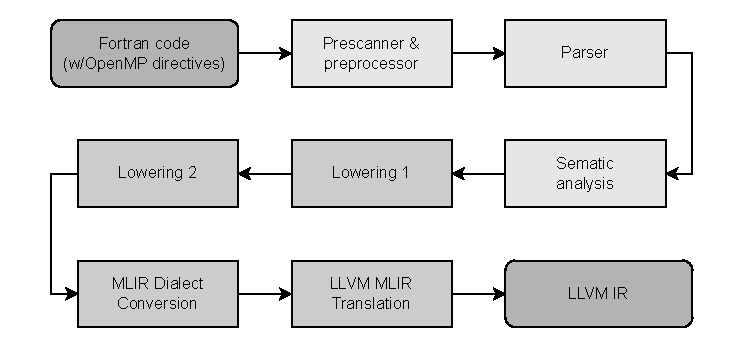
\includegraphics[width=\linewidth]{figures/flang_compiler_phases_overview.pdf}
\caption{Simplified overview of the compiler phases in the AMD Next Generation Fortran Compiler front-end.\label{fig:FlangCompilerPhases}}
\end{figure}

\begin{listing}[t]
\inputminted{Fortran}{code/tgt_loop.f90}
\caption{Example Fortran code with a \code{target teams loop} construct and a \code{map} clause.}
\label{lst:FortranExample}
\end{listing}

\begin{listing}[t]
\inputminted{text}{code/tgt_loop_cooked.f90}
\caption{Fortran code of Listing~\ref{lst:FortranExample} after preprocessing and prescanning.}
\label{lst:FortranExampleCooked}
\end{listing}

Figure~\ref{fig:FlangCompilerPhases} shows a simplified overview of the compiler pipeline of the AMD Flang compiler front-end up to LLVM \ac{IR} generation.
The same stages are also used by the AMD Next Generation Fortran Compiler front-end.
In the Prescanner \& Preprocessor stage, the lexical analysis and C-style processor produce a stream of characters of normalized Fortran source code. 
This code contains expanded preprocessor macros, including code resulting from \code{INCLUDE} statements. Unnecessary blank characters and comments are also removed in this stage (see Listing~\ref{lst:FortranExampleCooked}).
Compiler directives such as \code{!\$DIR} and the OpenMP directives introduced with \code{!\$OMP} remain in the stream of characters.
The parser and semantic analysis stages then construct a parse tree of the processed Fortran code and annotate it with semantic information (e.g., data types), which is known as the \ac{PFT}.
The \ac{PFT} contains all details about OpenMP directives, clauses, etc. as nodes in the tree.

\begin{listing}[t]
\inputminted{MLIR-lexer.py:MlirLexer -x}{code/tgt_loop_abridged.fir}
\caption{Abridged intermediate representation of the Fortran code in Listing~\ref{lst:FortranExample} with \acs{FIR} and OpenMP \acs{MLIR} dialects.}
\label{lst:FortranExampleFIR}
\end{listing}

% The parse tree is then gradually lowered into different levels of intermediate representation, depending on the needs of the applied transformation and optimization passes.

The \ac{PFT} is then gradually lowered using the \ac{MLIR} infrastructure~\cite{mlir}. The initial \ac{MLIR} representation obtained from the \ac{PFT} primarily contains operations from the \ac{HLFIR} and \ac{FIR} dialects of \ac{MLIR} (prefixed respectively with \code{hlfir} and \code{fir}).
These dialects provide operations and types that directly correspond to Fortran language concepts.
As the name suggests, the \code{hlfir} dialect is used to express higher level semantics of Fortran (e.g., array operations that can be used to optimize Fortran array statements) along with a type system to represent Fortran attributes for (dummy) variables.
The OpenMP constructs in the program are represented using operations from the OpenMP dialect (prefix \code{omp}).
This initial mix of \ac{MLIR} operations produced by the AMD Flang front-end then goes through multiple dialect conversion and transformation passes, which result in a final \ac{MLIR} module mainly holding \code{llvm}, \code{omp} and other low-level dialect operations for which direct translations to LLVM \ac{IR} are defined.
For example, the \code{DO} loop nest in Listing~\ref{lst:FortranExample} is expressed using \code{omp} dialect constructs that correspond to the OpenMP \code{target teams loop} construct as shown in Listing~\ref{lst:FortranExampleFIR}.

The \code{omp} dialect is designed to represent the directives and clauses defined by the OpenMP specification, so the \ac{MLIR} representation closely resembles the structure of the original program at a high-level.
Generally, each operation corresponds to a single directive, which can take multiple arguments to represent the various clauses supported by it.
A structured block associated with an OpenMP construct is represented in \ac{MLIR} through a region owned by that operation, resulting in a nesting structure that resembles the original program (e.g., see line~\ref{ln:SaxpyTargetStart} of Listing~\ref{lst:FortranExampleFIR}).
Combined constructs are split into each of their constituent parts while attaching the applicable clauses (explicit or implicit) to each leaf operation.
Loop-associated constructs are represented in the \code{omp} dialect by ``loop wrappers'', which are operations that meet stringent criteria:

\begin{itemize}
    \item they must have exactly one child operation;
    \item the nested operation must be an \code{omp.loop\_nest} or another compatible loop wrapper; and
    \item if there is more than one loop wrapper associated with an \code{omp.loop\_nest}, all wrappers must have the \code{omp.composite} attribute and represent a legal OpenMP composite construct (e.g., \code{do simd}).
\end{itemize}

For example, lines~\ref{ln:SaxpyParallelStart} to~\ref{ln:SaxpyParallelEnd} in Listing~\ref{lst:FortranExampleFIR} show how a \code{distribute parallel do} composite construct would be represented.
It includes the \code{omp.distribute} and \code{omp.wsloop} loop wrappers around a single \code{omp.loop\_nest} holding the loop body.
This also displays the one exception in the \code{omp} dialect where the original order of leaf constructs in a compound construct is not respected, which results in the \code{omp.parallel} operation being hoisted and made a parent of both loop wrappers.
Local variables introduced by clauses such as \code{private} or \code{map} are represented by entry block arguments to the code region owned by the corresponding \ac{MLIR} operation, and custom parsers and printers are provided to make the relationship between outside values and local ones explicit.
This is shown by the \code{omp.parallel private(...)} clause in the same example.

Contrary to the \code{hlfir} and \code{fir} dialects, even though the \code{omp} dialect features a relatively high level of abstraction, when it comes to translating \ac{MLIR} to LLVM \ac{IR}, it does not rely on conversions to other lower level dialects.
Instead of converting to other dialects with existing paths to LLVM \ac{IR}, the \code{omp} dialect can be directly translated to LLVM \ac{IR} through the use of the \textit{OpenMPIRBuilder}.
This utility, which is shared with Clang, helps reuse OpenMP-specific codegen logic between both frontends.
Once LLVM \ac{IR} is generated, this is handed to the compiler back-end for target code generation.

% OpenMP directives and clauses are reflected in this intermediate representation via an additional \ac{MLIR} dialect that mixes with \ac{HLFIR} and \ac{FIR}.
% Through these additional elements, the intermediate representation contains explicit information about  OpenMP directives and clauses in the code as well as their nesting structure.
% For instance, \code{DO} loop nest is associated with the corresponding OpenMP \code{target teams loop} construct (see Listing~\ref{lst:FortranExampleFIR}).
% Finally, the \ac{MLIR} code is transformed into regular LLVM \ac{IR} and is passed to the compiler back-end for target code generation.

%%%%%%%%%%%%%%%%%%%%%%%%%%%%%%%%%%%%%%%%%%%%%%%%%%%%%%%%%%%%%%%%%%%%%%%%%%%%%%%%%%%%%%%%%%%%%%%%%%%%%%%%%%%%
%%%%%%%%%%%%%%%%%%%%%%%%%%%%%%%%%%%%%%%%%%%%%%%%%%%%%%%%%%%%%%%%%%%%%%%%%%%%%%%%%%%%%%%%%%%%%%%%%%%%%%%%%%%%

\section{OpenMP Code Generation for GPU}
\label{sec:OpenMPCodeGen}

To generate code for device execution that adheres to the OpenMP semantics, the compiler has to perform these steps:

\begin{itemize}
\item identify implicitly and explicitly mapped variables for a \code{target} construct;
\item outline each \code{target} construct into a separate function;
\item generate boilerplate code to invoke the outlined function and pass data-mapping information to it; and
\item link the individual object files with host and device code to produce the final executable.
\end{itemize}

We will provide an overview of the above steps throughout the remainder of this section.

\subsection{OpenMP Data Mapping Analysis}
\label{sec:OpenMPDataMappingAnalysis}

Each list item in a \code{map} clause is processed individually to produce an individual \code{omp.map.info} operation in the intermediate representation. 
For a given \code{target} \code{map} clause, the \code{omp.map.info} operation encapsulates all the relevant information that is needed to map a variable onto the device.
This includes the \textit{map-type} modifier as well as the base address and bounds of the data to be mapped (see line~\ref{ln:SaxpyMapClause} of Listing~\ref{lst:FortranExample}).
For instance, the \textit{map-type} modifier \code{to} is represented as \code{map\_clauses(to)} in lines~\ref{ln:SaxpyMapInfoXStart}--\ref{ln:SaxpyMapInfoXEnd} in Listing~\ref{lst:FortranExampleFIR}.
The provided variable names (symbols), allow the compiler to gather the base address, type, and boundary data for the mapped data, populating the \code{var\_ptr} and \code{bounds} fields of the operation. 

In Listing~\ref{lst:FortranExample}, it can be seen that there are variables that are referenced within the \code{target} region which do not have a corresponding \code{map} clause (e.g., \code{y} and \code{a}).
As per the OpenMP specification~\cite{OARB24}, these variables are subject to implicit data mapping.
The compiler must analyze the code and create \code{omp.map.info} operations for these to capture the data for mapping operations. 
In Listing~\ref{lst:FortranExampleFIR}, one example of such an implicit map is in lines~\ref{ln:SaxpyMapInfoImplicitArrayStart}--\ref{ln:SaxpyMapInfoImplicitArrayEnd} with the \code{map\_clauses(implicit, ...)} attribute for the array \code{y}.
The capturing of variables occurs during the initial lowering of the \code{target} node after all present clauses have been processed, including any \code{map} clauses. 
At this stage the compiler has knowledge of what symbols have already been mapped to the device by the various OpenMP data movement clauses.

To generate the \code{omp.map.info} operation for a symbol, the compiler visits all of the symbols referenced within the \code{target} region and determines if they already appear in a \code{omp.map.info} operation (due to an explicit \code{map} clause or another \code{omp.map.info}-generating clauses). 
If not, the compiler begins the process of generating one, similar to what it would do for an explicit \code{map} clause.
The main difference is that the compiler must infer the correct \code{map\_type}, which in the explicit case is specified by the user on the \code{map} clause; in the implicit case it is the specified default behavior as per the OpenMP specification.
For example, Fortran arrays are treated as if they appeared in a \code{map} clause with a \code{map\_type} of \code{tofrom} (see Listing~\ref{lst:FortranExampleFIR}, lines~\ref{ln:SaxpyMapInfoImplicitArrayStart}--\ref{ln:SaxpyMapInfoImplicitArrayEnd}).
Fortran scalar data is treated as if they were specified with \code{map(to:...)} and a \code{firstprivate} clause.
This can be viewed as pass-by-copy, which results in giving them a \code{map\_type} of \code{to} and a \code{capture} field of \code{ByCopy} (see Listing~\ref{lst:FortranExampleFIR}, lines~\ref{ln:SaxpyMapInfoImplicitScalarStart}--\ref{ln:SaxpyMapInfoImplicitScalarEnd}). 

Additionally, \code{omp.map.info} operations are generated when allocatable variables appear in \code{private} or \code{firstprivate} clauses of the \code{target} construct.
In such cases, the descriptor of the allocatable variable is needed on the target side for initializing the private copy, so it is essential to map it using the \code{omp.map.info} operation.


\subsection{Kernel outlining}
\label{sec:KernelOutlining}

For OpenMP device code generation, the AMD Flang compiler utilizes a process that is very similar to the LLVM Clang compiler~\cite{antao2016offloading}.
There is one invocation of the compiler front-end for the host device and also one for each offloading target.
This results in multiple independent \ac{MLIR} modules obtained from the same source code, each holding an attribute that lowering and transformation passes use to produce compatible host and device LLVM \ac{IR}.

Target device modules are pruned early on in the process, removing all host-only functions except those holding target regions inside.
When compiling for a target device, at the \ac{MLIR} to LLVM \ac{IR} translation step, \code{omp.target} operations are identified and extracted from the host function where they are located into a new one.
These new outlined kernels, whose parameter list is based on the variables mapped into the target region, together with other device functions, are the only ones that remain in the resulting LLVM \ac{IR} module.
Host compilation (shown in Listing~\ref{lst:FortranExampleLLVMIR}) performs this kernel outlining process as well, but it maintains the original functions where target regions resided, replacing them with calls to the runtime \code{\_\_tgt\_target\_kernel} to offload their execution (lines~\ref{ln:SaxpyLLVMIRInvokeStart}--\ref{ln:SaxpyLLVMIRInvokeEnd}).

Whenever a kernel launch fails, the outlined host implementation for that target region is executed as a fallback (lines~\ref{ln:SaxpyLLVMIRHostStart}--\ref{ln:SaxpyLLVMIRHostEnd}).
The resulting host and device LLVM modules are later linked together following the process described in Section~\ref{sec:LinkingOpenMPHostandDeviceCode}.
% Except that in place of Clang's parsing and code generation we integrate analogous Flang components. 
% These are invoked through the Flang \code{ToolChain} which in turn is utilized by the existing Clang driver, which orchestrates the offloading compilation process.
% The first step generates the code for offload regions and the resulting (GPU) kernels that can be invoked from the host.
% The second step generates the code for host execution of the remaining code.
% In a later stage, the device binary code is embedded into the host code to create a single object file .
 
% Possible TODO: Perhaps add a section going into a bit of detail about the Fortran PFT -> MLIR process, Sergio or Krzysztof may be best for this, but I can likely do a fairly brief summary of it if we wish to add something here

\begin{listing}[t]
\inputminted{MLIR-lexer.py:MlirLexer -x}{code/tgt_loop_abridged.ll}
\caption{Abridged LLVM \ac{IR} of the Fortran code in Listing~\ref{lst:FortranExample} after host lowering has been performed.}
\label{lst:FortranExampleLLVMIR}
\end{listing}

% To generate GPU code for a \code{target} construct, the compiler performs a process called outlining that extracts the code associated with that \code{target} construct into a separate function.
% The compiler then creates a device function for the outlined code by feeding this outlined code into the code generator for the target device. 
% The outlined function is also processed by the code generator for the host to create the corresponding host version in case host fallback is needed (Listing~\ref{lst:FortranExampleLLVMIR}, lines~\ref{ln:SaxpyLLVMIRHostStart}--~\ref{ln:SaxpyLLVMIRHostEnd}) is needed.
% For additional book keeping in the runtime system, the compiler creates a unique ID of the transformed \code{target} construct.
% At the original code location, the compiler then emits code to call the runtime entry point \code{\_\_tgt\_target\_kernel} to invoke the device (see Listing~\ref{lst:FortranExampleLLVMIR}, lines~\ref{ln:SaxpyLLVMIRInvokeStart}--\ref{ln:SaxpyLLVMIRInvokeEnd}).

% In the former these functions become fallback functions, utilized if executing the device variant fails. 
% In the latter case the function becomes a kernel which contains specialized code for the target device, which in our case is a \ac{GPU}. 

% This involves generated code to perform data mapping according to the OpenMP semantics and code to invoke the kernel on the GPU via the runtime libraries. 

\todo{Kareem to expand on the late vs. early outling - 1 paragraph.}
% The outlining process in LLVM Flang is a form of late outlining, where the primary differentiation between host and device code occurs late in the compilation pipeline when the compiler is converting from \ac{MLIR} to LLVM \ac{IR}. 
% The code to be outlined as kernels are marked by the aforementioned OpenMP specification's \code{target} directive. 
% This directive can be combined with several other directives and clauses to make complex but performant programs. 
% Functions that can be invoked by the kernel must also be taken into consideration during this process and emitted for the device. 
% Such functions can be marked by users via the OpenMP \code{declare target} directive, or through implicit capture from function uses within the \code{target} region performed through Flang's \code{MarkDeclareTarget} \ac{MLIR} transformation pass. 

\subsection{Generating code for data mapping}
\label{sec:HandlingDataMapping}

% During the creation of the outlined kernel function from the \code{target} operation, an important consideration is how the list of \code{map.info} operations affects the kernel function on the device and the entry point on the host.

In an earlier phase, the compiler created \code{omp.map.info} statements in the \ac{IR} to capture mapped data needed for device execution (see Section~\ref{sec:OpenMPDataMappingAnalysis}).
This information needs to be passed to the runtime system to be able to perform necessary data transfers.
This is done via the \code{\%kernel\_args} argument of the \code{\_\_tgt\_target\_kernel} entry point (see Listing~\ref{lst:FortranExampleLLVMIR}).
The data structure consists of a structure of arrays, in which each array element corresponds to a mapped object with information about base pointer of the mapped object, its size, and additional flags for data-movement direction, etc.
The actual pointers to data that are used in the offloaded code are passed as pointer arguments to the outlined function.
At runtime, the offload library implementation will process the mapping information passed and the outlined function can access the mapped data via the passed pointers.

% During the \ac{MLIR} to LLVM \ac{IR} lowering of the \code{target} operation; prior to the generation of the kernel or entry point, the compiler gathers information from the \code{map.info} necessary for lowering of the kernel for each compiler pass. 
% The \code{map.info} operation conveys the minimum necessary information for this stage of the lowering, each pass still must perform some processing to meet the aforementioned requirements. 

% Populating the kernel argument data structure, requires the host pass calculates the size of data to be mapped, any possible offsets or required intermediate accesses the pointer fields may have and to compute the final map type. 

For each \code{omp.map.info} statement, the compiler generates LLVM \ac{IR} code to retrieve the base pointer as well as to compute its size and offset of the data to be mapped.
This is needed whenever the size of a data object is not statically known at compile time; for statically known information, the compiler pass computes these results ahead of time.
For instance, the compiler emits intermediate code to access the descriptor of arrays and read the dimensionality and extent in each dimension to compute the total number of array elements.
In \ac{FIR} this is reflected by the \code{omp.bounds} statement in lines~\ref{ln:SaxpyMapInfoXBoundsStart}--\ref{ln:SaxpyMapInfoXBoundsEnd} of Listing~\ref{lst:FortranExampleFIR} for the variable \code{x}.
In the lowered LLVM \ac{IR} code in Listing~\ref{lst:FortranExampleLLVMIR}, this corresponds to lines~\ref{ln:SaxpyLLVMIRBoundsXStart}--\ref{ln:SaxpyLLVMIRBoundsXEnd}.

% The calculation for the size of the data (in bytes) being mapped is trivial for non-arrays... . 
% In the case of array types the boundary data provided by the \code{omp.bounds} operation must be factored in...
% As we may not have the boundary data as a compile time constant, the compiler has to emit the instructions for the calculation and then insert the result to the data structure.

% Host: bit more detail on how it is done ... retrieve all map info, calculate size from type + bounds, calculate relevant offsets and apply to the base address when we're provided a slice, modify map type with relevant bits in certain cases but can mostly gloss over this and say it's a bitshift of all the specified maps with some minor runtime/lower level/situation specific flags, create parent <-> child relationships... maybe leave that out though it's a bit complicated and we don't really cover it in our example. Intermediate access above mainly referring to the ByRef/ByCopy semantics we carried over from Clang that the runtime requires

% Device: Details on how the varying capture types affect input argument access + Details on how the kernel arguments are decided upon.. bit simple, but deserves a sentence.

\subsection{Code generation for the OpenMP \code{reduction} clause}
\label{sec:OpenMPReduction}
The \code{reduction} clause specifies that a that a reduction operation should be performed on a value and what kind of reduction operation to perform, usually in the context of a loop.
Listing~\ref{lst:ReductionExample} shows a simple program using a reduction clause.
The AMD Flang compiler lowers the code to MLIR as shown in Listing~\ref{lst:MLIRReductionExample}.
The reduction operation itself is represented in MLIR as an \code{omp.declare\_reduction} operation.
In the simplest case, the \code{omp.declare\_reduction} operation contains an \code{init} block defining what the initial value should be for a reduction value and a \code{combiner} block which defines how to reduce two elements into one.
There are also optional blocks that handle allocation and deallocation of temporary data if needed.

In the executable code the reduction clauses are represented in \ac{MLIR} as inputs to operations. They contain essentially the same information as in the source code and specify which value should be reduced and which \code{omp.declare\_reduction} should be applied to the value.
For reductions that are both at the \code{teams} and workshare levels, the reductions map to the same value but go through various remappings to distinguish uses inside different regions. However, they are linked so that different levels of reductions operate on the same data. For example, on line~\ref{ln:ReductionRemap} the variable \code{\%21} gets remapped to \code{\%arg5}.

When generating LLVM \ac{IR} for the GPU reductions are split up between code that is generated for handling combining and copying data and calls to the device runtime library, which handles synchronization between threads, splits up the loop iterations, and calls the generated functions to perform combining and copying operations. This code generation is shared between Flang and Clang.

\begin{listing}[t]
\inputminted{Fortran}{code/tgt_reduction.f90}
\caption{Example Fortran code with the OpenMP \code{reduction} clause.}
\label{lst:ReductionExample}
\end{listing}

\begin{listing}[t]
\inputminted{MLIR-lexer.py:MlirLexer -x}{code/tgt_reduction_abridged.fir}
\caption{Listing~\ref{lst:ReductionExample} after initial lowering to \acs{MLIR}.}
\label{lst:MLIRReductionExample}
\end{listing}
% Codegen for GPU shared between clang and flang

\subsection{Linking OpenMP host and device code}
\label{sec:LinkingOpenMPHostandDeviceCode}
% Linking OpenMP host and device code is done using the Clang Linker Wrapper tool.
Both Flang and Clang compiler drivers use the Clang Linker Wrapper tool for linking together and optimizing host and device code code~\cite{LLVM25}.
This tool unifies the compilation procedure across hardware-specific toolchains and enables the generation of device code for multiple targets in a single compilation step.

The first step of the Clang Linker Wrapper is to extract the device LLVM IR code from the object files.
For each offload device type, the device LLVM \ac{IR} sections are combined with the LLVM \ac{IR} OpenMP device \ac{RTL} code.
Then, the LLVM \ac{IR} code is optimized using \ac{LTO} passes~\cite{clangLinkerWrapper}.
One of the optimization passes is the \ac{IPO} \textit{OpenMPOpt} pass, which understands the role of OpenMP runtime functions and can safely reduce OpenMP overhead~\cite{OpenMPOpt}.
The optimized device LLVM \ac{IR} is lowered into device-specific assembly, optimized by target-specific processes, and then embedded back into the host code before linking with other host libraries.

%%%%%%%%%%%%%%%%%%%%%%%%%%%%%%%%%%%%%%%%%%%%%%%%%%%%%%%%%%%%%%%%%%%%%%%%%%%%%%%%%%%%%%%%%%%%%%%%%%%%%%%%%%%%
%%%%%%%%%%%%%%%%%%%%%%%%%%%%%%%%%%%%%%%%%%%%%%%%%%%%%%%%%%%%%%%%%%%%%%%%%%%%%%%%%%%%%%%%%%%%%%%%%%%%%%%%%%%%

\section{Compiler Transformations to and between OpenMP Constructs}
\label{sec:CompilerTransOpenMP}

As mentioned in Section \ref{sec:LLVMFlangCompiler}, the AMD Flang compiler models Fortran programs using a mix of the \ac{FIR}, \ac{HLFIR}, and OpenMP \ac{MLIR} dialects.
% Different parts of the program are modeled using different dialects.
% For instance. the OpenMP directives and clauses are modeled using operations from the OMP dialect.
% Additionally, 
The \ac{MLIR} infrastructure allows for rewriting or transforming the \ac{IR} internally throughout the compiler pipelines using passes that create operations from the same or different dialect(s).
% This can take place within the same dialect, that is, the compiler rewrites a construct to use different operation(s) from the same dialect (e.g., OpenMP-to-OpenMP transformations).
% The compiler can also translate operations into a different dialect (e.g., \ac{FIR} to OpenMP \ac{IR} transformations).
In the following subsections, examples of such transformations implemented in the AMD Flang compiler are presented.
% All are currently implemented in the AMD Flang compiler.

\subsection{Automatically parallelizing \code{DO CONCURRENT} loops}
\label{sec:DCPar}

The Fortran \code{DO CONCURRENT}~\cite{F2023} construct allows users to write loops whose iterations can be executed in indeterminate order and express opportunities for code to execute concurrently.
\code{DO CONCURRENT}, however, does not specify how a loop should be parallelized or where the parallelized loop should be executed (e.g., CPU or GPU).
% Using the AMD Flang compiler, a user can control how \code{DO CONCURRENT} loops should behave.

\begin{listing}[t]
\inputminted{Fortran}{code/dc_saxpy.f90}
\caption{Example Fortran code with \code{do concurrent} loop.}
\label{lst:DCExample}
\end{listing}

\begin{listing}[t]
\inputminted{MLIR-lexer.py:MlirLexer -x}{code/dc_fir.mlir}
\caption{Listing~\ref{lst:DCExample} after lowering to \acs{FIR} and \acs{HLFIR} dialects.}
\label{lst:DCFIRExample}
\end{listing}

\begin{listing}[t]
\inputminted{MLIR-lexer.py:MlirLexer -x}{code/dc_omp.mlir}
\caption{Listing~\ref{lst:DCFIRExample} after lowering to OpenMP \ac{IR} on the CPU.}
\label{lst:DCOMPExample}
\end{listing}

\begin{listing}[t]
\inputminted{MLIR-lexer.py:MlirLexer -x}{code/dc_omp_device.mlir}
\caption{Listing~\ref{lst:DCFIRExample} after lowering to OpenMP \ac{IR} on the GPU.}
\label{lst:DCOMPDeviceExample}
\end{listing}

The \code{-fdo-concurrent-to-openmp} compiler option selects the compilation target for \code{DO CONCURRENT} loops.
The flag takes one of three possible arguments: \code{host}, \code{device}, or \code{none}.
Setting it to \code{host} or \code{device} tells the compiler that \code{DO CONCURRENT} loops should run in parallel on the CPU or the GPU, respectively.
The user can set the flag to \code{none} to prevent parallelization altogether.
Depending on the given command line flag, a different code translation from \ac{FIR} to the OpenMP \ac{IR} dialect is selected.

% This level of control is enabled by \ac{MLIR}'s ability to model program semantics using different dialects and to map or rewrite these program constructs from one dialect to another if needed.
% In this particular case, the compiler lowers a more abstract construct (\code{fir.do\_concurrent} \ac{MLIR} operations) to a more concrete set of constructs (the equivalent OMP dialect \ac{MLIR} constructs on the CPU or the GPU).

To further illustrate this, consider the Fortran code in Listing~\ref{lst:DCExample}.
Within the compiler pipeline, this loop is represented using the \ac{FIR} and \ac{HLFIR} dialects as shown in Listing~\ref{lst:DCFIRExample}.
At this stage of the pipeline, the loop's representation still maintains the original semantics of the input program, that is, the fact that this IR originated from a Fortran \code{DO CONCURRENT} construct.

How this loop is further lowered by the compiler can be controlled by the \code{-fdo-concurrent-to-openmp} flag.
For example, setting the flag to \code{host}, the \ac{FIR} and \ac{HLFIR} in Listing~\ref{lst:DCFIRExample} is lowered to an equivalent OpenMP program that parallelizes the loop on the CPU (Listing~\ref{lst:DCOMPExample}).
The transformed IR is mix of the three dialects: \code{fir}, \code{hlfir}, and \code{omp}.
Note, in particular, that the loop's body is not affected by the transformation; only the constructs that control how that loop will be executed.
The advantage of such progressive lowering is that the compiler can maintain the original program semantics as much as needed within the pipeline, which allows easier analyses and transformations.
The transformation pass that does the actual conversion from Fortran-specific constructs to OpenMP ones can be plugged into the compiler pipeline as late as needed, which allows Fortran-specific passes to finish their work before transforming \code{DO CONCURRENT} loops from the Fortran domain to the OpenMP domain.
Setting the \code{-fdo-concurrent-to-openmp} flag to \code{device} instead allows the user to map the loop to the device rather than the host.
Inside the compiler, this is done by rewriting the loop to the equivalent OpenMP constructs that launch a kernel on the GPU device that shares the iterations of the loop among the GPU's compute units (Listing~\ref{lst:DCOMPDeviceExample}).

The results of automatically parallelizing \code{DO CONCURRENT} on the CPU were reported in \cite{rouson2025automatically}.
GPU parallelization is still work-in-progress at the time of writing.

\subsection{Transforming the OpenMP \code{loop} directive}

\begin{listing}[t]
\inputminted{Fortran}{code/loop_dir_reduction.f90}
\caption{Example Fortran code with the OpenMP \code{loop} directive.}
\label{lst:LoopDirExample}
\end{listing}

\begin{listing}[t]
\inputminted{MLIR-lexer.py:MlirLexer -x}{code/loop_dir_reduction.mlir}
\caption{Listing~\ref{lst:LoopDirExample} after initial lowering to MLIR.}
\label{lst:LoopDirMLIRExample}
\end{listing}

\begin{listing}[t]
\inputminted{MLIR-lexer.py:MlirLexer -x}{code/loop_dir_simd.mlir}
\caption{Listing~\ref{lst:LoopDirMLIRExample} after lowering to \code{simd}.}
\label{lst:LoopDirSIMDExample}
\end{listing}

\begin{listing}[t]
\inputminted{MLIR-lexer.py:MlirLexer -x}{code/loop_dir_wsloop.mlir}
\caption{Listing~\ref{lst:LoopDirMLIRExample} after lowering to a work-sharing loop.}
\label{lst:LoopDirWSLoopExample}
\end{listing}

\begin{listing}[t]
\inputminted{Fortran}{code/loop_dir_teams_1.f90}
\caption{Example Fortran code with the OpenMP \code{loop} directive that can be mapped to a work-sharing loop.}
\label{lst:LoopDirTeamsExample1}
\end{listing}

\begin{listing}[t]
\inputminted{MLIR-lexer.py:MlirLexer -x}{code/loop_dir_teams_1.mlir}
\caption{Listing~\ref{lst:LoopDirTeamsExample1} after lowering.}
\label{lst:LoopDirTeamsMLIRExample1}
\end{listing}

\begin{listing}[t]
\inputminted{Fortran}{code/loop_dir_teams_2.f90}
\caption{Example Fortran code with the OpenMP \code{loop} directive that cannot be mapped to a work-sharing loop.}
\label{lst:LoopDirTeamsExample2}
\end{listing}

\begin{listing}[t]
\inputminted{MLIR-lexer.py:MlirLexer -x}{code/loop_dir_teams_1.mlir}
\caption{Listing~\ref{lst:LoopDirTeamsExample2} after lowering.}
\label{lst:LoopDirTeamsMLIRExample2}
\end{listing}

An OpenMP \code{loop} construct specifies that the logical iterations of the associated loops may execute concurrently~\cite{OARB21}.
The actual mapping/distribution of the associated loop's iterations across hardware resources depends on the region in which the \code{loop} directive is nested.
The OpenMP specification provides three possible mappings of a \code{loop} directive:
\begin{itemize}
    \item When it binds to a \code{teams} region, the loop's iterations are executed by the primary threads that execute the region.
    \item When it binds to a \code{parallel} region, the loop's iterations are executed by the team of threads in the \code{parallel} region.
    \item Otherwise, the loop is executed by a single thread.
\end{itemize}
During the initial stages of the compiler pipeline, the context (or binding region) of \code{loop} directives is ignored.
A \code{loop} directive is initially lowered as an \code{omp.loop} operation from the OpenMP \ac{MLIR} dialect (see Listings \ref{lst:LoopDirExample} and \ref{lst:LoopDirMLIRExample}).
For brevity, describing the \code{private} clause attached to the \code{omp.loop} directive is ignored; the \code{reduction} clause is discussed in Section \ref{sec:OpenMPReduction}.

Starting from the bottom item in the above list since it is the simplest case; \code{loop} directives could be simply serialized.
However, the AMD Flang compiler takes this a step further by converting \code{loop} directives in this case to corresponding OpenMP \code{simd} constructs (see Listing \ref{lst:LoopDirSIMDExample}).
The compiler (1) creates a new \code{omp.simd} \ac{MLIR} operation, (2) transfers the loop's body and attached clauses (i.e., \code{private} and \code{reduction}) to the new operation, and (3) deletes the original \code{omp.loop} operation.
Binding the \code{loop} directive to a \code{parallel} region (e.g., through tightly nesting the \code{loop} directive inside a \code{parallel} directive) results in different handling of the \code{omp.loop} op by the compiler.
Listing \ref{lst:LoopDirWSLoopExample} demonstrates this scenario where the same \code{omp.loop} in Listing \ref{lst:LoopDirMLIRExample} is now mapped to an \code{omp.wsloop} (i.e. a work-sharing loop) operation.
To perform this transformation, the compiler checks the surrounding context of the input \code{omp.loop} and, if it finds that the \code{omp.loop} operation is directly nested inside of an \code{omp.parallel} operation, then the \code{loop} directive is mapped to a work-sharing loop.

Handling the case where a \code{loop} directive binds to a \code{teams} region is more involved than the previous two cases.
To gain the most performance, a \code{loop} directive could be mapped to the \code{distribute parallel do} OpenMP composite construct.
However, this mapping is not always possible or safe to do.
In such cases, the compiler simply maps the \code{loop} directive to the \code{distribute} construct.
A \code{loop} construct with \code{teams} binding can be mapped to \code{distribute parallel do} only if:
\begin{itemize}
    \item it does not enclose another work-sharing loop; and
    \item it does not contain calls to functions that might themselves have nested parallelism.
\end{itemize}
Both restrictions are imposed to prevent nesting work-sharing loops.
At the time of writing, the first restriction is satisfied if a \code{loop} directive has \code{parallel} binding, whereas the second is satisfied if a call to a non-OpenMP runtime API is found in the loop's body.
Both restrictions can be made more general.
Listings \ref{lst:LoopDirTeamsExample1} and \ref{lst:LoopDirTeamsMLIRExample1} show an example where a \code{loop} directive can be mapped to a work-sharing loop due to not meeting any of the restrictions above.
Listings \ref{lst:LoopDirTeamsExample2} and \ref{lst:LoopDirTeamsMLIRExample2} show an example where a call to an unknown function \code{foo} inhibits converting the \code{loop} to a work-sharing loop.

Both transformations presented in Section~\ref{sec:DCPar} and in this section are examples of internal (i.e., \ac{MLIR} to \ac{MLIR}) transformations performed by the AMD Flang compiler. However, a few differences between the two stand out:
\begin{itemize}
    \item the former is driven by the user through a compiler flag while the latter is driven automatically by the compiler based on the nesting context/region; and
    \item the former transforms program constructs from one dialect to another while the latter transforms higher level constructs to lower level ones within the same dialect.
\end{itemize}

\subsection{Lowering of intrinsic arithmetic and mathematical functions to the GPU}
\label{sec:FortranIntrinsics}
Lowering of calls to intrinsic math functions is done via the \ac{MLIR} math dialect.
The math dialect operations are then lowered to calls to the ROCm\trademark math library or to LLVM \ac{IR} intrinsics if the operations are directly supported by the AMD GPU backend.
For complex types the intrinsic function calls are translated to the complex dialect and then lowered to ROCm\trademark math library calls.
The reason for going through the math and complex dialects instead of directly generating calls to \textit{libm} is that there is currently no \textit{libm} library available for the AMD GPU target and the ROCm\trademark math library function names differ from the \textit{libm} names. Another benefit is to allow more optimizations in \ac{MLIR} (e.g., constant folding).

\subsection{Handling Fortran arrays}
The Fortran language allows for declaring static and dynamic multi-dimensional arrays, bounds of which can be described by both positive and negative integers~\cite{F2023}.
In comparison to static arrays, which size needs to be determined at compilation time, the shape of dynamic arrays is set up during program runtime.
Listing \ref{lst:ArrayExample} presents an exemplary Fortran code that uses both types of arrays.

\begin{listing}[t]
\inputminted{Fortran}{code/arrays.f90}
\caption{Example Fortran code with static and dynamic arrays.}
\label{lst:ArrayExample}
\end{listing}

Declaration of dynamic arrays are tagged with the keyword \code{allocatable}.
The Fortran standard guarantees that all allocatable objects are safely removed when the program goes out of the scope of the variable declaration.
The function \code{allocate} is responsible for allocating sufficient memory for a given array shape.
In comparison to the \code{malloc} function in the C standard library, the Fortran allocate function not only reserves required memory, but also stores information about allocated array size and base pointer in an array descriptor: a Flang runtime structure describing dynamically allocated objects.
Static arrays do not require descriptors because information about the shape of the array is explicitly defined in Fortran source code, and the AMD Flang compiler can use parsed data to calculate the addresses of array elements without loading data from an array descriptor.

The reference to array elements is denoted in the same way for static and dynamic arrays in the Fortran source code.
Despite the same notation, the generated codes are different.
The compiler decides which instruction needs to be generated during subsequent phases of \ac{MLIR} lowering.
Initially, the \ac{PFT} sub-trees that describe a reference to an element of the array are converted into \code{hlfir.designate} operations.
The arguments of these operations correspond to the \ac{MLIR} variable that describes the array and the \ac{MLIR} index~\cite{LLVM25}.
The \code{hlfir.designate} operation does not differentiate notation between static and dynamic arrays, and it is lowered to the FIR operations that describe how the address of a given array element is calculated.
Listing \ref{lst:FIRStaticArray} presents \code{fir} operations generated for an \code{hlfir.designate} operation to a static array.


\begin{listing}[t]
\inputminted{MLIR-lexer.py:MlirLexer -x}{code/FIR_static_array.mlir}
\caption{Simplified FIR code for a static array.}
\label{lst:FIRStaticArray}
\end{listing}

The \code{fir.array\_coor} operation takes an argument with the memory address of the first element, another stating the declared shape of the array and one to denote the index of the search array element.

\begin{listing}[t]
\inputminted{MLIR-lexer.py:MlirLexer -x}{code/FIR_dynamic_array.mlir}
\caption{Simplified FIR code for a dynamic array.}
\label{lst:FIRDynamicArray}
\end{listing}

The calculation of the memory address where a given element of the dynamic array is stored is more complicated, and it is illustrated by the simplified \ac{FIR} code in Listing \ref{lst:FIRDynamicArray}.
It shows that both the dimensions and the base address of a dynamically allocated array are calculated based on information stored in the array descriptor.
The \code{fir.box\_addr} operation corresponds to the calculation of the memory address where the array is allocated, while the \code{fir.box\_dims} operation reads the bounds of the array.
The \code{fir.shape\_shift} operation is a \ac{FIR}-specific operation that converts a set of numbers into a \ac{FIR} abstract shape object.
Finally, when all required data is loaded from the descriptor, it is possible to determine the pointer to a given element of the dynamically allocated array using an \code{fir.array\_coor} operation~\cite{LLVM25}.

\subsection{Comparison of the code generated by Clang and Flang}
The way array elements are accessed is the same for code executed on a GPU and on a CPU.
However, the handling of descriptors requires more load operations, which can lead to a higher number of registers being used and increased memory usage.
High register occupancy and increased memory usage can lead to significantly slower code, especially for GPUs, where memory bandwidth is the primary factor limiting the efficiency of calculations.
That's why the register usage metric provides information about the quality of the generated code for GPUs.
A smaller number of used registers corresponds to better optimized code.
Table \ref{tab:registerUsage} presents the number of \acp{VGPR} and \acp{SGPR} used for different types of OpenMP GPU kernels.
The number of registers required for Fortran code with static arrays, when compiled by AMD Flang at the -O3 optimization level, is comparable to equivalent C code compiled by AMD Clang for the MI300 GPU.
The comparable number of registers used for Fortran code with static arrays and equivalent C code at the -O3 optimization level indicates that the Fortran code can be heavily optimized by the existing passes, which were primarily written for the optimization of C OpenMP code.

\begin{table}
    \small
    \caption{Usage of registers for statically and dynamically allocated arrays.}
    \label{tab:registerUsage}
    \begin{tabular}{|c|c|c|c|}\hline
         Optimization &  Static arrays &  Dynamic arrays & Static arrays\\
         level        &  \acsp{SGPR}/\acsp{VGPR}    & \acsp{SGPR}/\acsp{VGPR}     &\acsp{SGPR}/\acsp{VGPR}  \\
                      &  (AMD Flang)   &  (AMD Flang)    & (AMD Clang) \\
        \hline\hline
         -O1&  40/32&  40/33& 18/6\\
         \hline
         -O2&  21/10&  26/10& 18/6\\
         \hline
         -O3&  19/10&  28/10& 18/6\\
         \hline
    \end{tabular}

\end{table}

\subsection{Limiting dynamic memory allocation on the GPU}
Dynamic memory allocation (i.e., using \code{malloc}) is managed by the \ac{OS}.
Since the GPU cannot directly request such service from the \ac{OS}, calls to \code{malloc} on the GPU have to be routed to the host first; which in turn requests the memory allocation from the \ac{OS}.
Once the allocation is successful and the host receives a pointer to the memory block, it then transfers the ownership of that block to the GPU, completing the the allocation process.
This communication mechanism between the CPU and GPU is implemented through an \ac{RPC} call from the GPU to the CPU (\cite{gpulibc}).
Such an \ac{RPC} communication mechanism comes with a cost, which can be alleviated by moving allocations to the stack when that transformation is profitable.

\begin{listing}[t]
\inputminted{Fortran}{code/temp_array.f90}
\caption{Example Fortran code with a temporary array.}
\label{lst:TempArrayExample}
\end{listing}

\begin{listing}[t]
\inputminted{MLIR-lexer.py:MlirLexer -x}{code/temp_array_heap.mlir}
\caption{Listing \ref{lst:TempArrayExample} with LLVM Flang's default behavior.}
\label{lst:TempArrayHeapExample}
\end{listing}

\begin{listing}[t]
\inputminted{MLIR-lexer.py:MlirLexer -x}{code/temp_array_stack.mlir}
\caption{Listing \ref{lst:TempArrayExample} with AMD Flang's stack-arrays optimization.}
\label{lst:TempArrayStackExample}
\end{listing}

One situation where such transformation is beneficial is for temporary arrays.
Listing \ref{lst:TempArrayExample} provides an example where a \code{target} region includes an allocation of a temporary array.
Here, \code{[x, x*2]} constructs a two-element array which is then assigned to \code{my\_array}.
By default, the AMD Flang compiler allocates these temporary arrays on the heap (for the sake of brevity, the reasons for such design choice are not discussed here).
Listing \ref{lst:TempArrayHeapExample} shows such default behavior.
In particular, the \code{fir.allocmem} and \code{fir.destroy} \ac{MLIR} operations correspond to dynamic memory allocation (a call to \code{malloc}) and deallocation (a call to \code{free}), respectively.
To allocate the temporary array on the stack instead; AMD Flang's \textit{stack-arrays} pass was extended to process OpenMP regions and the pass is used when compiling for the GPU.
The result of this transformation is shown in Listing \ref{lst:TempArrayStackExample}.

%%%%%%%%%%%%%%%%%%%%%%%%%%%%%%%%%%%%%%%%%%%%%%%%%%%%%%%%%%%%%%%%%%%%%%%%%%%%%%%%%%%%%%%%%%%%%%%%%%%%%%%%%%%%
%%%%%%%%%%%%%%%%%%%%%%%%%%%%%%%%%%%%%%%%%%%%%%%%%%%%%%%%%%%%%%%%%%%%%%%%%%%%%%%%%%%%%%%%%%%%%%%%%%%%%%%%%%%%

\section{Conclusions}
\label{sec:Conclusions}

\todo{
Dan to write this part - 2 paragraphs
\begin{itemize}
    \item Short summary of the paper - 1 paragraph
    \item Future work - 1 paragraph
    \begin{itemize}
        \item Implement missing OpenMP features up to OpenMP 6.0, give few examples
        \item Finish DO CONCURRENT
        \item Performance improvements
    \end{itemize}
    \item Upstream implementation to LLVM project 
\end{itemize}
}

\section*{List of Acronyms}

\begin{acronym}[paper]
\acro{AST}[AST]{Abstract Syntax Tree}
\acro{API}[API]{application programming interface}
\acro{CCD}[CCD]{compute complex die}
\acro{CFD}[CFD]{computational fluid dynamics}
\acro{CU}[CU]{compute unit}
\acro{FIR}[FIR]{Fortran intermediate representation}
\acro{GPU}[GPU]{graphics processing unit}
\acro{HLFIR}[HLFIR]{high-level Fortran intermediate representation}
\acro{HPC}[HPC]{high-performance computing}
\acro{IPO}[IPO]{interprocedural optimization}
\acro{IR}[IR]{intermediate representation}
\acro{LTO}[LTO]{link time optimization}
\acro{MLIR}[MLIR]{multi-level intermediate representation}
\acro{XCD}[XCD]{accelerator complex die}
\acro{WENO}[WENO]{weighted essentially non-oscillatory}
\acro{SDK}[SDK]{software development kit}
\acro{HIP}[HIP]{Heterogeneous-computing Interface for Portability}
\acro{IFA}[IFA]{isolated from above}
\acro{PFT}[PFT]{Pre-FIR Tree}
\acro{RTL}[RTL]{run-time library}
\end{acronym}

%%%%%%%%%%%%%%%%%%%%%%%%%%%%%%%%%%%%%%%%%%%%%%%%%%%%%%%%%%%%%%%%%%%%%%%%%%%%%%%%%%%%%%%%%%%%%%%%%%%%%%%%%%%%
%%%%%%%%%%%%%%%%%%%%%%%%%%%%%%%%%%%%%%%%%%%%%%%%%%%%%%%%%%%%%%%%%%%%%%%%%%%%%%%%%%%%%%%%%%%%%%%%%%%%%%%%%%%%

\section*{Acknowledgments}
Copyright 2025 Advanced Micro Devices, Inc.
AMD, the AMD Arrow logo, Instinct, Radeon, and EPYC, and combinations thereof are trademarks of Advanced Micro Devices, Inc.
Other product names used in this publication are for identification purposes only and may be trademarks of their respective companies.

\printbibliography

\end{document}
